\documentclass[aspectratio=169]{beamer}

% =================================================================
%  Pointers and Strings in C
%  A beginner-friendly Beamer deck (fully self-contained: all
%  figures / diagrams drawn with TikZ, so it compiles anywhere).
%  Style mirrors "c-programming-intro.tex".
% =================================================================

% -------------------------------------------------
% Theme and packages
% -------------------------------------------------
\usetheme{Madrid}
\usecolortheme{default}

\usepackage{amsmath}
\usepackage{amssymb}
\usepackage{bm}
\usepackage{listings}
\usepackage{tikz}
\usepackage{array}
\usepackage{booktabs}
\usepackage{tabularx}
\usepackage{ragged2e}
\usepackage{xcolor}

\usetikzlibrary{shapes.geometric, arrows.meta, positioning, calc, fit, backgrounds}

% -------------------------------------------------
% Colour palette
% -------------------------------------------------
\definecolor{cAccent}{RGB}{0,102,153}     % teal-blue accent
\definecolor{cBox}{RGB}{28,31,42}          % dark box
\definecolor{cGreen}{RGB}{34,139,34}
\definecolor{cRed}{RGB}{178,34,34}
\definecolor{cOrange}{RGB}{204,102,0}
\definecolor{cPurple}{RGB}{102,45,145}
\definecolor{cGrayBg}{RGB}{245,246,248}
\definecolor{codebg}{RGB}{248,248,244}
\definecolor{codekw}{RGB}{0,0,180}
\definecolor{codecomment}{RGB}{0,130,0}
\definecolor{codestr}{RGB}{170,55,20}

% Beamer colour tweaks (match a Madrid-style accent)
\setbeamercolor{structure}{fg=cAccent}
\setbeamertemplate{frametitle continuation}{%
	\ifnum\insertcontinuationcount>1\space(cont...)\fi
}
\setbeamertemplate{navigation symbols}{}
\setbeamertemplate{caption}[numbered]

% -------------------------------------------------
% Listings style for C code
% -------------------------------------------------
\lstdefinestyle{cstyle}{
	language=C,
	backgroundcolor=\color{codebg},
	basicstyle=\ttfamily\footnotesize,
	keywordstyle=\color{codekw}\bfseries,
	commentstyle=\color{codecomment}\itshape,
	stringstyle=\color{codestr},
	numbers=none,
	numberstyle=\tiny\color{gray},
	numbersep=8pt,
	showstringspaces=false,
	breaklines=true,
	frame=single,
	rulecolor=\color{gray!50},
	tabsize=2,
	columns=fullflexible,
	keepspaces=true,
	literate={~}{{$\sim$}}1
}
\lstset{style=cstyle}

% Handy TikZ node styles
\tikzset{
	startstop/.style={rectangle, rounded corners=10pt, minimum width=2.4cm, minimum height=0.8cm, text centered, align=center, draw=black, fill=cAccent!25},
	process/.style  ={rectangle, minimum width=2.6cm, minimum height=0.8cm, text centered, align=center, text width=2.8cm, draw=black, fill=blue!8},
	io/.style       ={trapezium, trapezium left angle=70, trapezium right angle=110, minimum width=2.2cm, minimum height=0.8cm, text centered, align=center, draw=black, fill=cOrange!20},
	decision/.style ={diamond, aspect=2, minimum width=2.4cm, minimum height=0.9cm, text centered, text width=2.2cm, draw=black, fill=cGreen!18, inner sep=1pt},
	flowarrow/.style={-{Stealth[length=2.5mm]}, thick},
	% memory-cell helpers
	acell/.style={draw=black, minimum width=1.05cm, minimum height=1.0cm, text centered, font=\small, fill=blue!8},
	varbox/.style={draw=black, minimum width=1.6cm, minimum height=1.0cm, text centered, font=\small, fill=blue!8},
	ptrbox/.style={draw=black, minimum width=1.6cm, minimum height=1.0cm, text centered, font=\small, fill=cGreen!14},
}

\setbeamertemplate{footnote}{%
	\parindent 0em
	\noindent
	\raggedright
	\insertfootnotemark\insertfootnotetext\par
}

% -------------------------------------------------
% Title information
% -------------------------------------------------
\title[Pointers \& Strings]{Pointers and Strings in C}
\subtitle{Addresses, Pointer Arithmetic, and Character Strings}
\author[Amit Kumar Singh]{}
\institute[]{
	Amit Kumar Singh \\
	\vspace{0.1cm}
	Assistant Professor (ECE) \\
	\vspace{0.05cm}
	School of Naval Architecture and Ocean Engineering\\
	\vspace{0.05cm}
	Indian Maritime University Visakhapatnam Campus, Sabbavaram Mandal\\
	\vspace{0.05cm}
	Visakhapatnam, Andhra Pradesh -- 531~035\\
	\vspace{0.25cm}
	amitkumarsingh@imu.ac.in
}
\date[Programming in C]{\today}

\begin{document}

	%------------------------------------------------
	\begin{frame}
		\titlepage
	\end{frame}

	%------------------------------------------------
	\begin{frame}{Outline}
		\small
		\begin{columns}[T,onlytextwidth]
			\hspace{0.8cm}
			\begin{column}{0.49\textwidth}
				\tableofcontents[hideallsubsections, sections={1-4}]
			\end{column}
			\hspace{0.8cm}
			\begin{column}{0.42\textwidth}
				\tableofcontents[hideallsubsections, sections={5-8}]
			\end{column}
		\end{columns}
	\end{frame}

	% =================================================================
	\section{Introduction to Pointers}
	% =================================================================
	\begin{frame}{Why Do We Need Pointers?}
		\begin{block}{Motivation}
			Every variable lives at some \textbf{address} in memory. A \textbf{pointer} lets us
			work with that address directly --- a powerful idea that unlocks much of C.
		\end{block}
		\begin{columns}[T]
			\begin{column}{0.5\textwidth}
				\begin{block}{Pointers make possible}
					\begin{itemize}\small
						\item Functions that \textbf{change} their caller's variables (call by reference).
						\item Efficient handling of \textbf{arrays} and \textbf{strings}.
						\item \textbf{Dynamic memory} (\texttt{malloc}, \texttt{free}).
						\item Building \textbf{linked lists}, trees, and other structures.
					\end{itemize}
				\end{block}
			\end{column}
			\begin{column}{0.5\textwidth}
				\begin{block}{The core idea}
					\small A pointer is just a variable whose \emph{value} is a \textbf{memory address}
					--- it ``points to'' where some data lives.
				\end{block}
				\centering\footnotesize Master pointers and the rest of C becomes much clearer.
			\end{column}
		\end{columns}
	\end{frame}

	\begin{frame}{Memory, Addresses, and What a Pointer Is}
		\begin{block}{Definition}
			A \textbf{pointer} is a variable that stores the \textbf{address} of another variable.
		\end{block}
		\vspace{0.15cm}
		\centering
		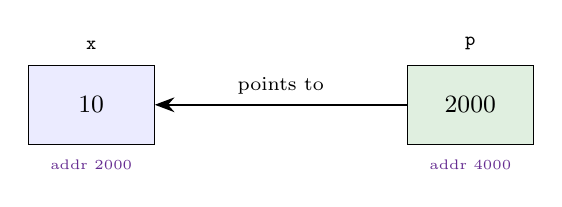
\begin{tikzpicture}[font=\small]
			\node[varbox] (x) {10};
			\node[font=\scriptsize, above=2pt of x] {\texttt{x}};
			\node[font=\tiny, text=cPurple, below=2pt of x] {addr 2000};
			\node[ptrbox, right=3.2cm of x] (p) {2000};
			\node[font=\scriptsize, above=2pt of p] {\texttt{p}};
			\node[font=\tiny, text=cPurple, below=2pt of p] {addr 4000};
			\draw[flowarrow] (p.west) -- node[above, font=\scriptsize]{points to} (x.east);
		\end{tikzpicture}
		\vspace{0.2cm}
		\begin{itemize}\small
			\item \texttt{x} holds the value \texttt{10} at address \texttt{2000}.
			\item \texttt{p} holds \texttt{2000} --- the \emph{address of} \texttt{x} --- so \texttt{p} points to \texttt{x}.
		\end{itemize}
	\end{frame}

	% =================================================================
	\section{Declaration and Initialization}
	% =================================================================
	\begin{frame}[fragile]{Declaring Pointer Variables}
		\begin{block}{Syntax}
			\centering \texttt{data\_type\ *pointer\_name;}
		\end{block}
		\begin{columns}[T]
			\begin{column}{0.52\textwidth}
				\begin{lstlisting}
int   *p;      /* p points to an int   */
float *fp;     /* fp points to a float */
char  *cp;     /* cp points to a char  */
int   *q = NULL;  /* empty, safe start */
				\end{lstlisting}
			\end{column}
			\begin{column}{0.48\textwidth}
				\begin{itemize}\small
					\item The \texttt{*} marks the variable as a \textbf{pointer}.
					\item The \textbf{type} says what it points to --- an \texttt{int *} points to an \texttt{int}.
					\item An uninitialized pointer holds \textbf{garbage}; set it to \texttt{NULL} until it has a real target.
				\end{itemize}
			\end{column}
		\end{columns}
	\end{frame}

	\begin{frame}[fragile]{Initializing Pointers}
		\begin{columns}[T]
			\begin{column}{0.52\textwidth}
				\begin{lstlisting}
int  x = 10;
int *p;

p = &x;          /* p gets address of x */
printf("%d", *p); /* prints 10          */
				\end{lstlisting}
				\vspace{0.1cm}
				\footnotesize A pointer is initialized with an \textbf{address} --- usually \texttt{\&someVariable}.
			\end{column}
			\begin{column}{0.48\textwidth}
				\centering
				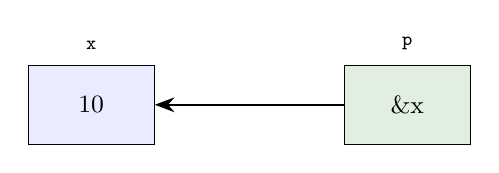
\begin{tikzpicture}[font=\small]
					\node[varbox] (x) {10};
					\node[font=\scriptsize, above=2pt of x] {\texttt{x}};
					\node[ptrbox, right=2.4cm of x] (p) {\&x};
					\node[font=\scriptsize, above=2pt of p] {\texttt{p}};
					\draw[flowarrow] (p.west) -- (x.east);
				\end{tikzpicture}
				\vspace{0.2cm}
				\begin{block}{Danger}
					\small Never dereference an \textbf{uninitialized} or \texttt{NULL} pointer --- it crashes the program.
				\end{block}
			\end{column}
		\end{columns}
	\end{frame}

	% =================================================================
	\section{Pointer Operators}
	% =================================================================
	\begin{frame}{The Two Pointer Operators: \texttt{\&} and \texttt{*}}
		\renewcommand{\arraystretch}{1.35}
		\centering
		\begin{tabular}{@{}clp{6.3cm}@{}}
			\toprule
			\textbf{Operator} & \textbf{Name} & \textbf{Meaning} \\
			\midrule
			\texttt{\&} & Address-of      & gives the \emph{address} of a variable: \texttt{\&x} \\
			\texttt{*}  & Dereference     & gives the \emph{value stored at} an address: \texttt{*p} \\
			\bottomrule
		\end{tabular}
		\vspace{0.35cm}
		\begin{block}{They are opposites}
			\centering \texttt{p = \&x;} \; means ``\texttt{p} = address of \texttt{x}''\\[3pt]
			\texttt{*p} \; then means ``the value at that address'' \; $=$ \; \texttt{x}
		\end{block}
		\centering\footnotesize So \texttt{*(\&x)} is just \texttt{x} again.
	\end{frame}

	\begin{frame}[fragile]{Reading and Writing Through a Pointer}
		\begin{columns}[T]
			\begin{column}{0.55\textwidth}
				\begin{lstlisting}
int  x = 5;
int *p = &x;

printf("%d\n", x);    /* 5             */
printf("%p\n", p);    /* address of x  */
printf("%d\n", *p);   /* 5  (via ptr)  */

*p = 20;              /* write through p */
printf("%d\n", x);    /* 20  - x changed! */
				\end{lstlisting}
			\end{column}
			\begin{column}{0.45\textwidth}
				\begin{itemize}\small
					\item \texttt{*p} \textbf{reads} the value \texttt{p} points to.
					\item \texttt{*p = 20;} \textbf{writes} to that same location --- so \texttt{x} becomes \texttt{20}.
				\end{itemize}
				\begin{block}{Key insight}
					\small Because \texttt{p} points \emph{at} \texttt{x}, changing \texttt{*p} changes \texttt{x} itself.
				\end{block}
			\end{column}
		\end{columns}
	\end{frame}

	% =================================================================
	\section{Pointer Expressions and Arithmetic}
	% =================================================================
	\begin{frame}{Pointer Arithmetic: Moving in Steps of the Type}
		\begin{block}{The rule}
			Adding \texttt{1} to a pointer moves it forward by \textbf{one element}, not one byte:
			\centering $\texttt{p + 1} \;\Rightarrow\; \text{address} + 1 \times \texttt{sizeof(type)}$
		\end{block}
		\vspace{0.1cm}
		\centering
		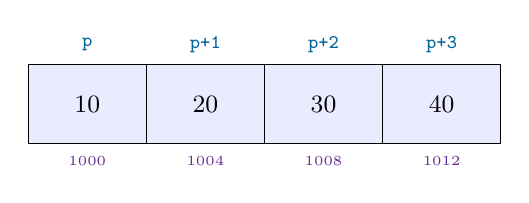
\begin{tikzpicture}
			\foreach \val/\idx/\addr in {10/0/1000, 20/1/1004, 30/2/1008, 40/3/1012} {
				\node[acell, minimum width=1.5cm] (c\idx) at (\idx*1.5,0) {\val};
				\node[font=\tiny, text=cPurple] at (\idx*1.5,-0.72) {\addr};
			}
			\node[font=\scriptsize, text=cAccent] at (0,0.75) {\texttt{p}};
			\node[font=\scriptsize, text=cAccent] at (1.5,0.75) {\texttt{p+1}};
			\node[font=\scriptsize, text=cAccent] at (3.0,0.75) {\texttt{p+2}};
			\node[font=\scriptsize, text=cAccent] at (4.5,0.75) {\texttt{p+3}};
		\end{tikzpicture}
		\vspace{0.15cm}
		\centering\footnotesize For an \texttt{int} (4 bytes), \texttt{p+1} is 4 addresses later --- the compiler scales automatically.
	\end{frame}

	\begin{frame}[fragile]{Valid Pointer Expressions}
		\begin{columns}[T]
			\begin{column}{0.48\textwidth}
				\renewcommand{\arraystretch}{1.25}
				\centering
				\begin{tabular}{@{}ll@{}}
					\toprule
					\textbf{Expression} & \textbf{Effect} \\
					\midrule
					\texttt{p + n} & move forward \texttt{n} elements \\
					\texttt{p - n} & move back \texttt{n} elements \\
					\texttt{p++}   & advance to next element \\
					\texttt{p2 - p1} & count elements between \\
					\texttt{p1 == p2} & compare two pointers \\
					\bottomrule
				\end{tabular}
			\end{column}
			\begin{column}{0.52\textwidth}
				\begin{lstlisting}
int a[3] = {10, 20, 30};
int *p = a;        /* -> a[0] */

printf("%d\n", *p);       /* 10 */
printf("%d\n", *(p + 1)); /* 20 */
p++;                      /* -> a[1] */
printf("%d\n", *p);       /* 20 */
				\end{lstlisting}
				\footnotesize \textbf{Not allowed:} adding two pointers, or multiplying/dividing them.
			\end{column}
		\end{columns}
	\end{frame}

	% =================================================================
	\section{Pointers and Arrays}
	% =================================================================
	\begin{frame}{The Relationship Between Pointers and Arrays}
		\begin{block}{An array name is a pointer to its first element}
			For \texttt{int a[5];}, the name \texttt{a} is the address of \texttt{a[0]}. So an array and a
			pointer are deeply related.
		\end{block}
		\vspace{0.1cm}
		\centering
		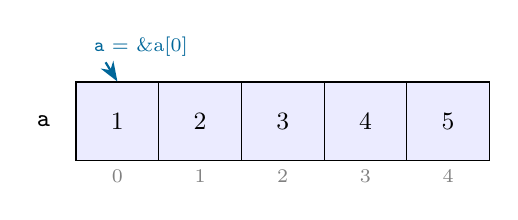
\begin{tikzpicture}
			\foreach \val/\idx in {1/0, 2/1, 3/2, 4/3, 5/4} {
				\node[acell] (c\idx) at (\idx*1.05,0) {\val};
				\node[font=\scriptsize, text=gray] at (\idx*1.05,-0.7) {\idx};
			}
			\node[left=0.2cm of c0, font=\ttfamily\small] {a};
			\draw[flowarrow, cAccent] (-0.15,0.75) -- (c0.north);
			\node[font=\scriptsize, text=cAccent] at (0.3,0.95) {\texttt{a} $=$ \&a[0]};
		\end{tikzpicture}
		\vspace{0.1cm}
		\begin{block}{The four equivalent forms}
			\centering \texttt{a[i]} \;$\equiv$\; \texttt{*(a + i)} \;$\equiv$\; \texttt{*(p + i)} \;$\equiv$\; \texttt{p[i]} \quad (where \texttt{p = a})
		\end{block}
	\end{frame}

	\begin{frame}[fragile]{Traversing an Array with a Pointer}
		\begin{columns}[T]
			\begin{column}{0.55\textwidth}
				\begin{lstlisting}
int  a[5] = {1, 2, 3, 4, 5};
int *p;

/* p walks from a[0] up to a[4] */
for (p = a; p < a + 5; p++)
    printf("%d ", *p);
/* prints: 1 2 3 4 5 */
				\end{lstlisting}
			\end{column}
			\begin{column}{0.45\textwidth}
				\begin{itemize}\small
					\item \texttt{p = a} starts the pointer at \texttt{a[0]}.
					\item \texttt{p++} steps to the next element.
					\item \texttt{a + 5} is one past the last element --- the loop stops there.
				\end{itemize}
				\begin{block}{Note}
					\small Indexing (\texttt{a[i]}) and pointer walking (\texttt{*p}) do the same job --- choose whichever reads more clearly.
				\end{block}
			\end{column}
		\end{columns}
	\end{frame}

	% =================================================================
	\section{Introduction to Strings}
	% =================================================================
	\begin{frame}{What is a String in C?}
		\begin{block}{Concept}
			C has no separate ``string'' type. A \textbf{string} is simply a \textbf{char array}
			ending with a special \textbf{null character} \texttt{'\textbackslash 0'} that marks where it stops.
		\end{block}
		\vspace{0.1cm}
		\centering
		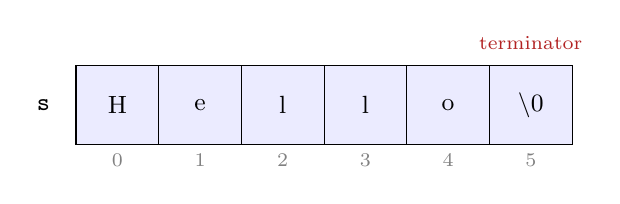
\begin{tikzpicture}
			\foreach \ch/\idx in {H/0, e/1, l/2, l/3, o/4, {$\backslash$0}/5} {
				\node[acell] (c\idx) at (\idx*1.05,0) {\ch};
				\node[font=\scriptsize, text=gray] at (\idx*1.05,-0.7) {\idx};
			}
			\node[left=0.2cm of c0, font=\ttfamily\small] {s};
			\node[font=\scriptsize, text=cRed, above=2pt of c5] {terminator};
		\end{tikzpicture}
		\vspace{0.15cm}
		\begin{itemize}\small
			\item \texttt{"Hello"} needs \textbf{6} bytes: 5 letters $+$ the \texttt{'\textbackslash 0'}.
			\item Library functions rely on \texttt{'\textbackslash 0'} to know where the text ends.
		\end{itemize}
	\end{frame}

	\begin{frame}[fragile]{Declaring, Initializing, and Reading Strings}
		\begin{columns}[T]
			\begin{column}{0.55\textwidth}
				\begin{lstlisting}
char s1[] = "Hello";   /* size 6: 5 + '\0' */
char s2[10] = "Hi";    /* extra space kept  */
char *s3 = "World";    /* pointer to literal */

printf("%s\n", s1);    /* print with %s     */

char name[20];
scanf("%s", name);        /* stops at space  */
fgets(name, 20, stdin);   /* safer full line */
				\end{lstlisting}
			\end{column}
			\begin{column}{0.45\textwidth}
				\begin{itemize}\small
					\item \texttt{"..."} automatically appends the \texttt{'\textbackslash 0'} for you.
					\item Print a whole string with \texttt{\%s}; the array name is the address.
					\item \texttt{scanf("\%s", name)} needs \textbf{no} \texttt{\&} (the name is already an address) and stops at whitespace.
					\item \texttt{fgets} is safer --- it limits the length and reads spaces too.
				\end{itemize}
			\end{column}
		\end{columns}
	\end{frame}

	% =================================================================
	\section{String Handling Library}
	% =================================================================
	\begin{frame}{The String Handling Library: \texttt{<string.h>}}
		\begin{block}{Ready-made string functions}
			Include \texttt{\#include <string.h>} to use these common operations.
		\end{block}
		\renewcommand{\arraystretch}{1.3}
		\centering
		\begin{tabular}{@{}llp{5.7cm}@{}}
			\toprule
			\textbf{Function} & \textbf{Purpose} & \textbf{Example} \\
			\midrule
			\texttt{strlen(s)}      & length (excludes \texttt{'\textbackslash 0'}) & \texttt{strlen("Hi")} $\rightarrow$ 2 \\
			\texttt{strcpy(d, s)}   & copy \texttt{s} into \texttt{d}   & \texttt{strcpy(d,"Hi")} \\
			\texttt{strcat(d, s)}   & append \texttt{s} to \texttt{d}   & \texttt{"Hi"+"There"} \\
			\texttt{strcmp(a, b)}   & compare (0 if equal)              & \texttt{strcmp("a","a")} $\rightarrow$ 0 \\
			\texttt{strchr(s, c)}   & find a character                  & first \texttt{'l'} in \texttt{s} \\
			\texttt{strstr(s, t)}   & find a substring                  & \texttt{"lo"} inside \texttt{s} \\
			\bottomrule
		\end{tabular}
		\vspace{0.15cm}
		\centering\footnotesize The \texttt{strn...} variants (\texttt{strncpy}, \texttt{strncat}, \texttt{strncmp}) take a length limit and are safer.
	\end{frame}

	\begin{frame}[fragile]{String Manipulation in Action}
		\begin{columns}[T]
			\begin{column}{0.56\textwidth}
				\begin{lstlisting}
#include <stdio.h>
#include <string.h>

int main(void)
{
    char a[20] = "Hello";
    char b[20] = "World";

    printf("%lu\n", strlen(a));  /* 5 */
    strcat(a, b);                /* HelloWorld */
    printf("%s\n", a);
    printf("%d\n", strcmp("ab","ac")); /* < 0 */
    strcpy(b, "Hi");             /* b = "Hi" */
    printf("%s\n", b);
    return 0;
}
				\end{lstlisting}
			\end{column}
			\begin{column}{0.44\textwidth}
				\begin{block}{What happens}
					\small
					\begin{itemize}
						\item \texttt{strlen} counts letters (5).
						\item \texttt{strcat} joins \texttt{b} onto \texttt{a}.
						\item \texttt{strcmp} returns $<0$, $0$, or $>0$.
						\item \texttt{strcpy} overwrites \texttt{b}.
					\end{itemize}
				\end{block}
				\centering\footnotesize Ensure the destination array is \textbf{big enough} to hold the result.
			\end{column}
		\end{columns}
	\end{frame}

	\begin{frame}[fragile]{String Conversion Functions}
		\begin{block}{Turning text into numbers (and back)}
			Text like \texttt{"1234"} is \emph{not} the number 1234. Conversion functions bridge the gap.
		\end{block}
		\begin{columns}[T]
			\begin{column}{0.5\textwidth}
				\renewcommand{\arraystretch}{1.25}
				\centering
				\begin{tabular}{@{}lll@{}}
					\toprule
					\textbf{Function} & \textbf{Header} & \textbf{Does} \\
					\midrule
					\texttt{atoi} & \texttt{stdlib.h} & text $\to$ int \\
					\texttt{atof} & \texttt{stdlib.h} & text $\to$ double \\
					\texttt{atol} & \texttt{stdlib.h} & text $\to$ long \\
					\texttt{sprintf} & \texttt{stdio.h} & number $\to$ text \\
					\texttt{sscanf}  & \texttt{stdio.h} & text $\to$ values \\
					\bottomrule
				\end{tabular}
			\end{column}
			\begin{column}{0.5\textwidth}
				\begin{lstlisting}
#include <stdlib.h>
char num[] = "1234";
char pi[]  = "3.14";

int    n = atoi(num);  /* 1234 */
double d = atof(pi);   /* 3.14 */

printf("%d\n", n + 1); /* 1235 */
printf("%.2f\n", d*2); /* 6.28 */
				\end{lstlisting}
			\end{column}
		\end{columns}
	\end{frame}

	% =================================================================
	\section{C Program Examples}
	% =================================================================
	\begin{frame}[fragile]{Example 1: Swap Two Numbers (Call by Reference)}
		\begin{columns}[T]
			\begin{column}{0.56\textwidth}
				\begin{lstlisting}
#include <stdio.h>

void swap(int *a, int *b)  /* take addresses */
{
    int t = *a;
    *a = *b;               /* edit caller's data */
    *b = t;
}

int main(void)
{
    int x = 3, y = 7;
    swap(&x, &y);          /* pass addresses */
    printf("%d %d\n", x, y);  /* 7 3 */
    return 0;
}
				\end{lstlisting}
			\end{column}
			\begin{column}{0.44\textwidth}
				\begin{block}{Why pointers are essential here}
					\small Without pointers, a function gets \emph{copies} and cannot change the originals.
					Passing \texttt{\&x} and \texttt{\&y} lets \texttt{swap} reach the real variables.
				\end{block}
				\centering\footnotesize Output:\; \fbox{\texttt{7 3}}
			\end{column}
		\end{columns}
	\end{frame}

	\begin{frame}[fragile]{Example 2: String Length Without the Library}
		\begin{columns}[T]
			\begin{column}{0.56\textwidth}
				\begin{lstlisting}
#include <stdio.h>

int my_strlen(char *s)
{
    int len = 0;
    while (s[len] != '\0')  /* until terminator */
        len++;
    return len;
}

int main(void)
{
    char text[] = "Pointer";
    printf("Length = %d\n", my_strlen(text));
    return 0;
}
				\end{lstlisting}
			\end{column}
			\begin{column}{0.44\textwidth}
				\begin{block}{The idea}
					\small Walk the character array one step at a time and \textbf{stop at} \texttt{'\textbackslash 0'},
					counting as we go. This is exactly what \texttt{strlen} does internally.
				\end{block}
				\centering\footnotesize Output:\; \fbox{\texttt{Length = 7}}
			\end{column}
		\end{columns}
	\end{frame}

	\begin{frame}[fragile]{Example 3: Reverse a String In Place}
		\begin{columns}[T]
			\begin{column}{0.58\textwidth}
				\begin{lstlisting}
#include <stdio.h>
#include <string.h>

int main(void)
{
    char s[] = "abcd";
    int  i, j;
    char t;

    for (i = 0, j = strlen(s) - 1; i < j; i++, j--) {
        t = s[i];          /* swap the ends */
        s[i] = s[j];
        s[j] = t;
    }
    printf("%s\n", s);     /* dcba */
    return 0;
}
				\end{lstlisting}
			\end{column}
			\begin{column}{0.42\textwidth}
				\begin{block}{How it works}
					\small Two indices move inward from both ends, swapping characters until they meet
					in the middle.
				\end{block}
				\centering\footnotesize
				\texttt{a b c d} $\rightarrow$ \texttt{d c b a}\\[4pt]
				Output:\; \fbox{\texttt{dcba}}
			\end{column}
		\end{columns}
	\end{frame}

	\begin{frame}{Summary \& What Comes Next}
		\begin{columns}[T]
			\begin{column}{0.5\textwidth}
				\begin{block}{You now know}
					\begin{itemize}\small
						\item What a pointer is and why C needs them.
						\item Declaring, initializing, and dereferencing pointers.
						\item The \texttt{\&} and \texttt{*} operators.
						\item Pointer expressions and arithmetic.
						\item How arrays and pointers relate (\texttt{a[i] = *(a+i)}).
						\item Strings as null-terminated char arrays and \texttt{<string.h>}.
					\end{itemize}
				\end{block}
			\end{column}
			\begin{column}{0.5\textwidth}
				\begin{block}{Practice}
					\begin{itemize}\small
						\item Count vowels in a string.
						\item Concatenate two strings without \texttt{strcat}.
						\item Use a pointer to find an array's maximum.
					\end{itemize}
				\end{block}
				\begin{block}{Coming up}
					\small Dynamic memory (\texttt{malloc}/\texttt{free}), structures, and linked lists.
				\end{block}
			\end{column}
		\end{columns}
	\end{frame}

	%------------------------------------------------
	\begin{frame}
		\centering
		\Huge Thank You
		\vspace{0.5cm}

		\normalsize Questions?
	\end{frame}

	%------------------------------------------------
\end{document}
